\section{Call of Duty Black Ops 2}

\begin{figure}[htbp]
\begin{center}
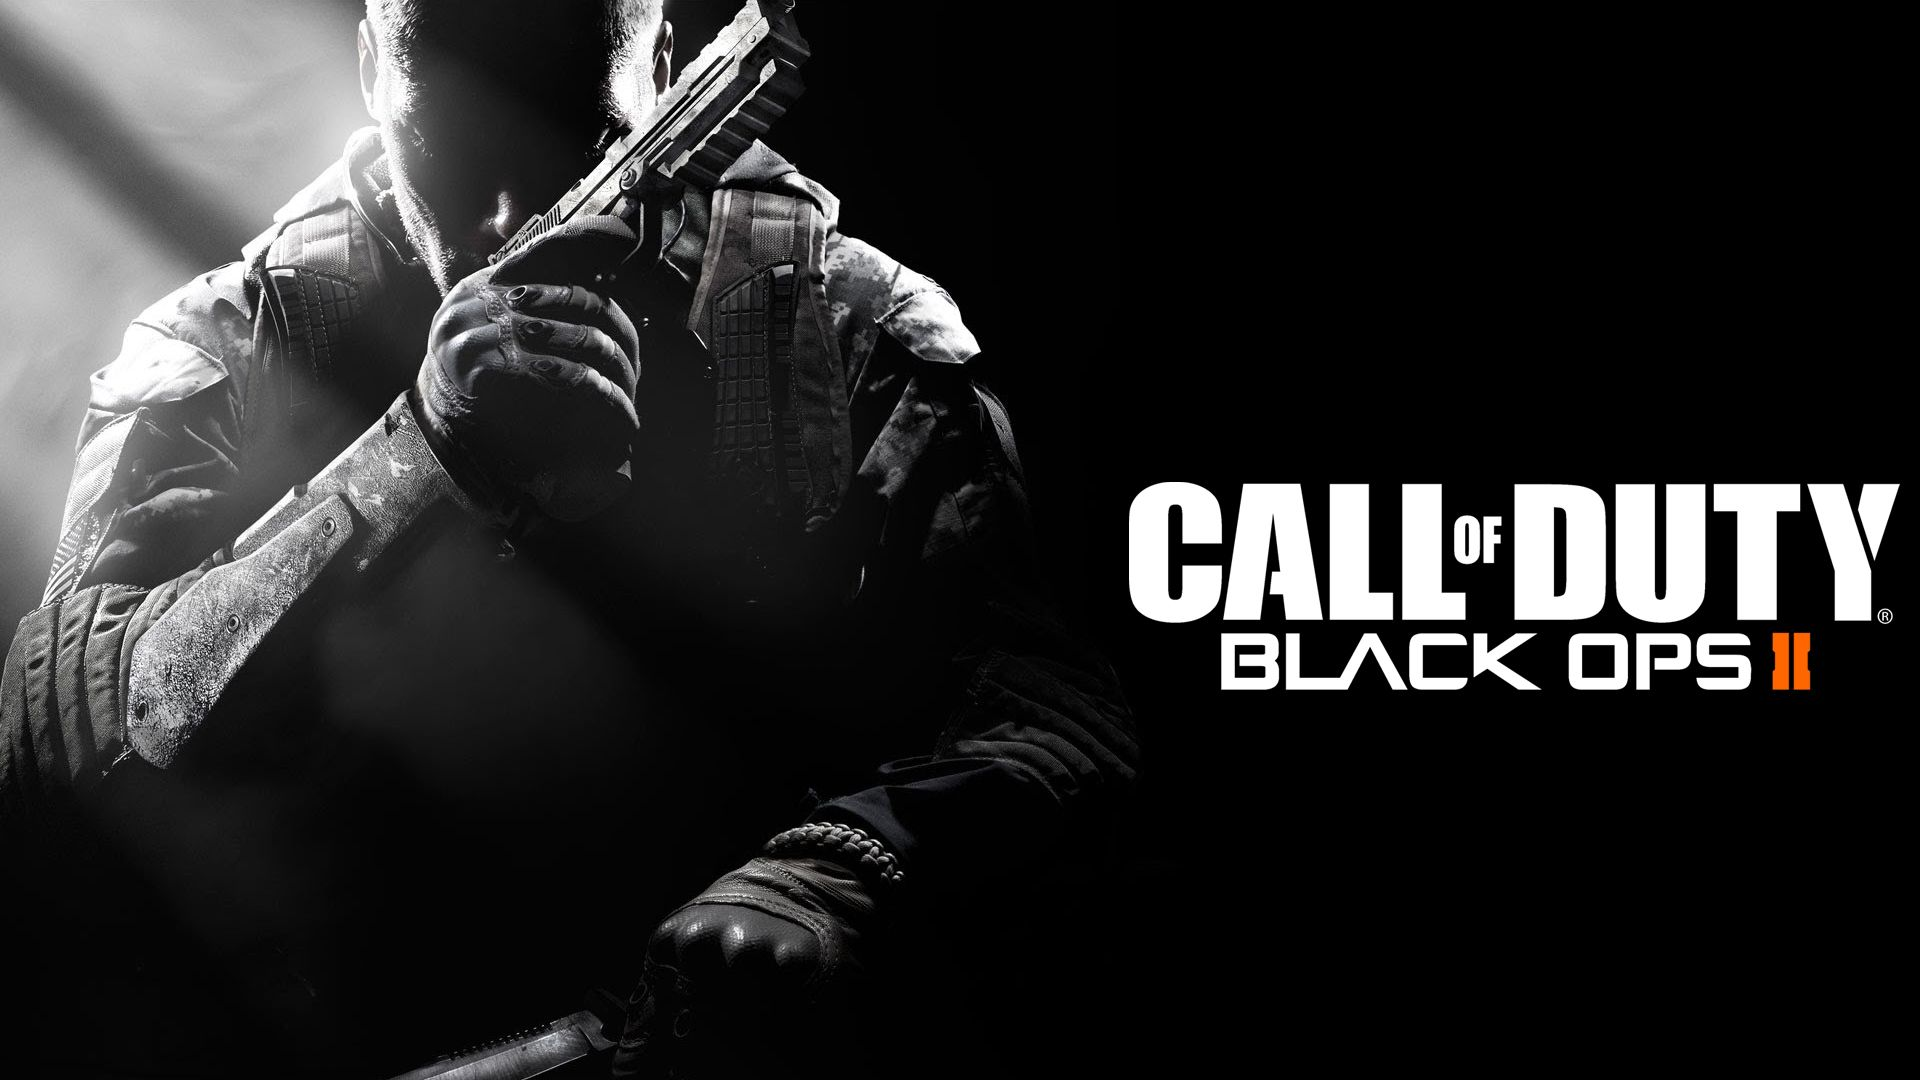
\includegraphics[width=.60\textwidth]{./imagenes/black.jpg}
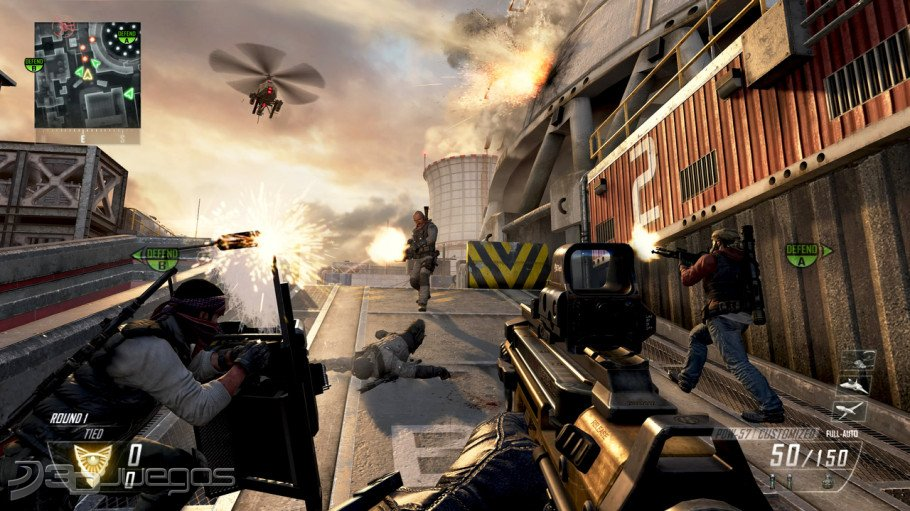
\includegraphics[width=.60\textwidth]{./imagenes/black2.jpg}
\caption{Call of Duty Black Ops 2}
\label{Call of Duty Black Ops 2}
\end{center}
\end{figure}
Call of Duty Black Ops 2\footnote{\url{http://www.callofduty.com/blackops2}}Es el primer juego de la saga Call of Duty que toma lugar en el futuro del 2025, donde China y Estados Unidos se han envuelto en una Segunda Guerra fría, a diferencia de su predecesor Call of Duty: Modern Warfare 3 que tomaba lugar en el futuro del 2016 en la Tercera Guerra Mundial . El 13 de Noviembre salió oficialmente a la venta esta nueva entrega de la saga y fue aceptada por una gran cantidad de gamers ya que fue pensado para el multijugador complementado por un modo campaña y un modo zombies que esta vez es más completo que nunca.

La premisa del juego es que eres un sargento llamado David Manson que con la ayuda de viejos aleados, deben detener la segunda guerra fría que Raúl Menéndez quiere provocar.

\subsubsection{¿Por qué es uno de mis juegos favoritos?}
\begin{itemize}
\item[Adrian Aguilar]Es un juego que requiere agilidad en movimientos ya sea en campaña o en multijugador. El modo campaña tiene varias dificultades y también tiene varias escenas donde debemos vencer al ejército enemigo. El modo multijugador es el más interesante ya que puedes desafiar a varias personas y demostrarles que eres el mejor. Este modo lo puedes jugar en solitario (FREE FOR ALL) o también en grupos (TEAM DEATHMACH) donde por cada muerte que realices te darán puntos y subirás de nivel desbloqueándose una gran variedad de armamento. El juego además tiene un modo llamado Zombies que es multijugador el cual se juega en grupos (un grupo de zombies y otro de soldados). La finalidad es matar a los zombies pero esto no es fácil ya que ellos tienen la habilidad de ser veloces y si te lastiman te convierten en uno de ellos.
\end{itemize}
